\subsubsection{Scénario Cockburn}
\textbf{Cas d'utilisation: }Rentrer

\textbf{Acteur primaire:} Le conducteur

\textbf{Pré-condition: } La voie est libre et ouvertre.
 
\textbf{Post-condition: } Le systeme de paiement est opérationnel


\textbf{Scénario primaire: } \\
    \textbf{1.} La boucle détecte le véhicule.\\
    \textbf{2.} La boucle envoi l’information à la borne.\\
    \textbf{3.} La borne détermine le type de véhicule. Le type est autorisé. \\
    \textbf{4.} La borne affiche le montant sur l'écran.\\

\textbf{Variantes:}\\
    \textbf{1a.} La boucle ne repère pas le véhicule, l’utilisateur ne peut pas passer. L’utilisateur doit appeler le technicien. Fin scénario.\\
    \textbf{3a.}L’opérateur repère un véhicule prioritaire en urgence. L’opérateur ouvre la barrière manuellement. Fin scénario. \\
    \textbf{3b.} Le type de véhicule n’est pas autorisé. Le conducteur appelle le technicien.\\
    \textbf{4a.} La borne n’affiche pas le montant, l’utilisateur ne peut pas payer , le conducteur appelle le technicien.\\
\newpage    
\subsubsection{Diagramme d'activité}
\begin{figure}[!htb]
    \centering
    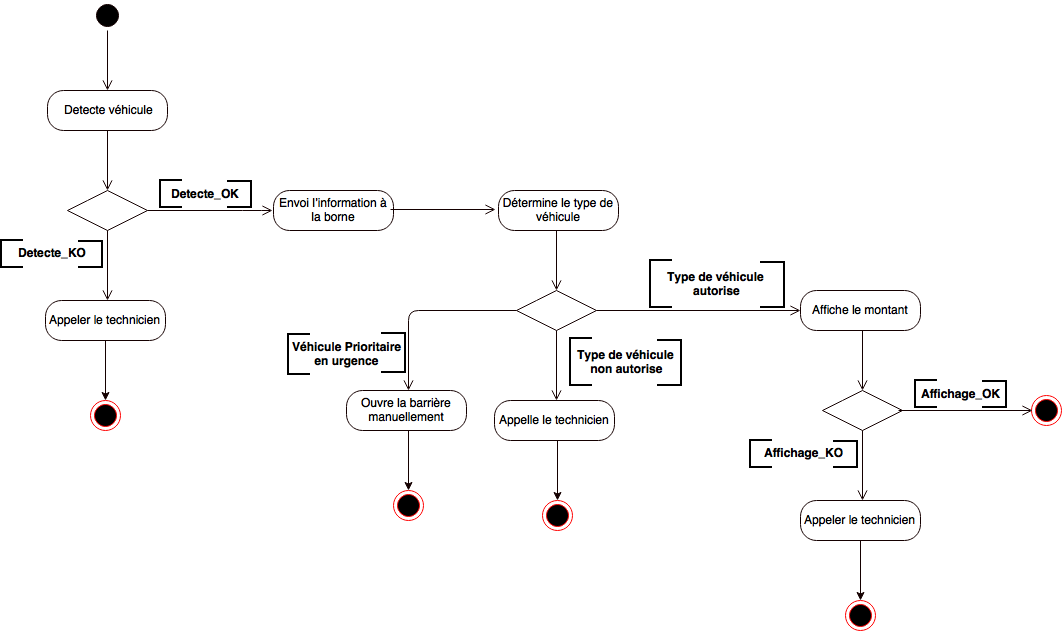
\includegraphics[scale=0.45, angle = 90]{02_Desenvolvimento/TD2/images/DARentrer.png}
    \caption{Diagramme d'activité - Rentrer}
    \label{fig:DARentrer}
\end{figure}
\newpage
\subsubsection{Collaboration}
\begin{figure}[!htb]
    \centering
    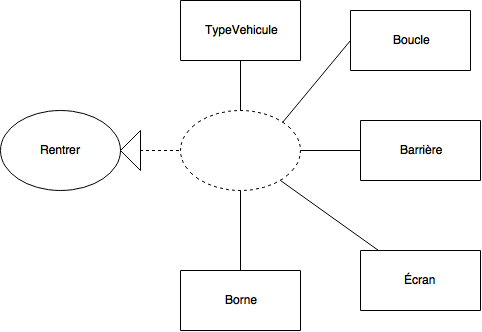
\includegraphics[scale=0.7]{02_Desenvolvimento/TD2/images/ColaRentrer.png}
    \caption{Collaboration - Rentrer}
    \label{fig:DARentrer}
\end{figure}
\newpage
\subsubsection{Diagramme de séquence ( à revisiter )}
\begin{figure}[!htb]
    \centering
    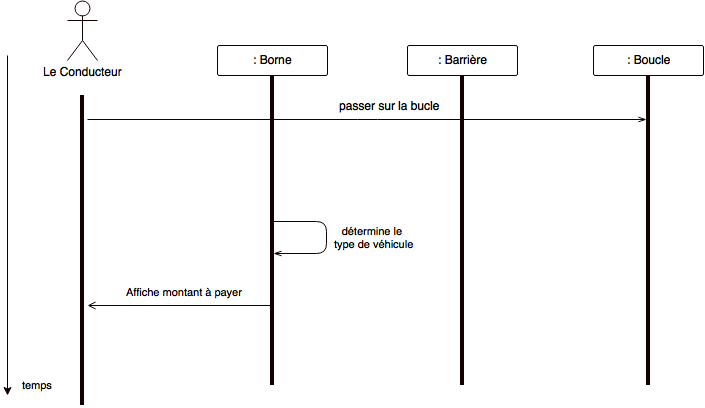
\includegraphics[scale=0.5]{02_Desenvolvimento/TD2/images/DSRentrer.png}
    \caption{Diagramme de séquence à revisiter  - Rentrer}
    \label{fig:DARentrer}
\end{figure}
\subsubsection{Diagramme de séquence}
\begin{figure}[!htb]
    \centering
    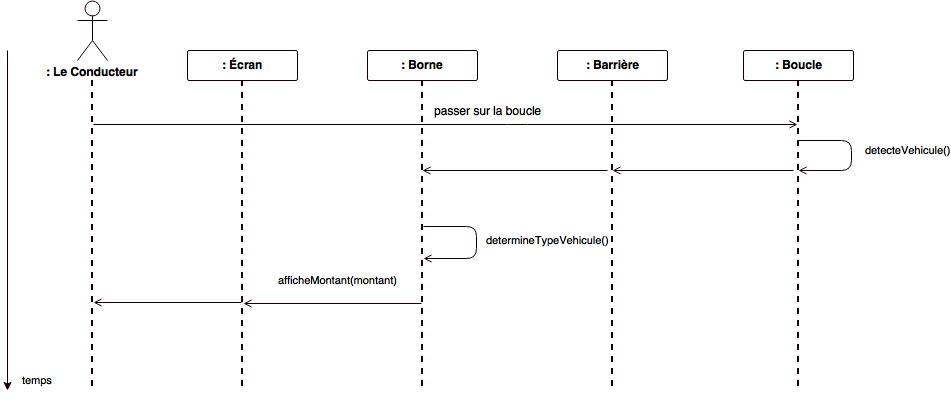
\includegraphics[scale=0.5]{02_Desenvolvimento/TD2/images/v2-DSRentrer.png}
    \caption{Diagramme de séquence - Rentrer}
    \label{fig:DARentrer}
\end{figure}